\documentclass[tikz,border=5pt]{standalone}
\usepackage[T1]{fontenc}
\usepackage{lmodern,amsmath,amssymb}
\usetikzlibrary{arrows.meta,calc,positioning,fit,backgrounds,shapes.geometric,matrix,decorations.pathreplacing,patterns}
\definecolor{ink}{gray}{0.08}
\definecolor{wash}{gray}{0.965}
\definecolor{soft}{gray}{0.45}
\tikzset{box/.style={draw=ink,line width=.65pt,fill=white,align=center,inner sep=4pt,outer sep=0pt,font=\small},flow/.style={draw=ink,line width=.65pt,-{Latex[length=1.8mm,width=1.3mm]},rounded corners=2pt},annotation/.style={font=\scriptsize,text=soft,align=center},groupbox/.style={draw=soft,dashed,line width=.45pt,fill=wash}}
\begin{document}
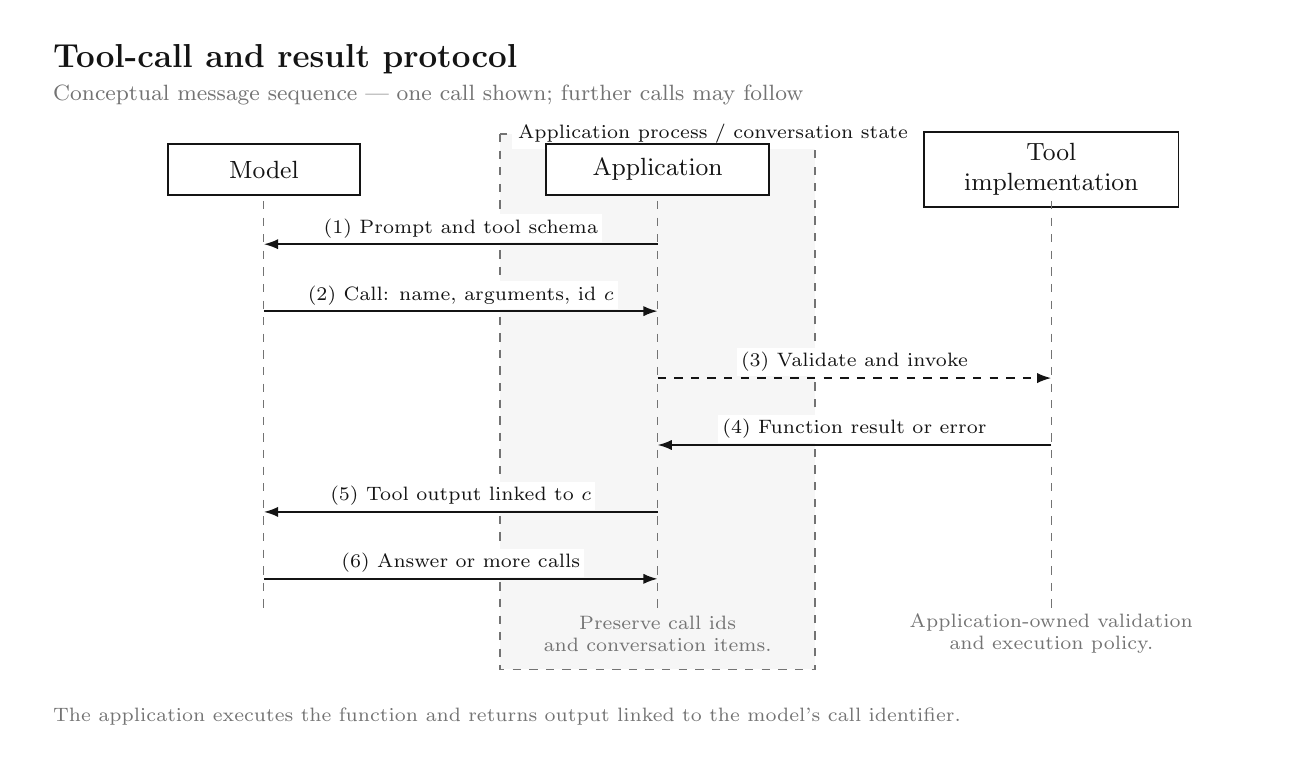
\begin{tikzpicture}[x=1cm,y=-1cm,font=\rmfamily,text=ink]

\path[use as bounding box] (0,0) rectangle (16,9);
\node[anchor=west,font=\large\bfseries] at (.2,.4) {Tool-call and result protocol};
\node[anchor=west,font=\footnotesize,text=soft] at (.2,.85) {Conceptual message sequence | one call shown; further calls may follow};
\begin{pgfonlayer}{background}
\draw[groupbox] (6.0,1.35) rectangle (10.0,8.15);
\node[anchor=west,font=\scriptsize,fill=white,inner sep=2pt] at (6.15,1.35) {Application process / conversation state};
\end{pgfonlayer}
\node[box,minimum width=2.4cm,minimum height=0.65cm,text width=2.15cm] (model) at (3.0,1.8) {Model};
\node[box,minimum width=2.8cm,minimum height=0.65cm,text width=2.55cm] (app) at (8.0,1.8) {Application};
\node[box,minimum width=3.2cm,minimum height=0.85cm,text width=2.95cm] (tool) at (13.0,1.8) {Tool\\implementation};
\begin{pgfonlayer}{background}
\end{pgfonlayer}
\foreach \x in {3,8,13} {\draw[soft,dashed,line width=.4pt] (\x,2.2) -- (\x,7.4);}
\draw[flow] (8,2.75) -- (3,2.75);
\node[font=\scriptsize,fill=white,inner sep=1.5pt,anchor=south] at (5.5,2.73) {(1) Prompt and tool schema};
\draw[flow] (3,3.6) -- (8,3.6);
\node[font=\scriptsize,fill=white,inner sep=1.5pt,anchor=south] at (5.5,3.58) {(2) Call: name, arguments, id $c$};
\draw[flow,dashed] (8,4.45) -- (13,4.45);
\node[font=\scriptsize,fill=white,inner sep=1.5pt,anchor=south] at (10.5,4.430000000000001) {(3) Validate and invoke};
\draw[flow] (13,5.3) -- (8,5.3);
\node[font=\scriptsize,fill=white,inner sep=1.5pt,anchor=south] at (10.5,5.28) {(4) Function result or error};
\draw[flow] (8,6.15) -- (3,6.15);
\node[font=\scriptsize,fill=white,inner sep=1.5pt,anchor=south] at (5.5,6.130000000000001) {(5) Tool output linked to $c$};
\draw[flow] (3,7.0) -- (8,7.0);
\node[font=\scriptsize,fill=white,inner sep=1.5pt,anchor=south] at (5.5,6.98) {(6) Answer or more calls};
\node[annotation,anchor=center,text width=3.55cm] at (8.0,7.7) {Preserve call ids\\and conversation items.};
\node[annotation,anchor=center,text width=3.7cm] at (13.0,7.7) {Application-owned validation\\and execution policy.};
\node[anchor=west,align=left,font=\scriptsize,text=soft,text width=15.6cm] at (.2,8.75) {The application executes the function and returns output linked to the model's call identifier.};
\end{tikzpicture}
\end{document}
